% Generar PNG
% convert -density 300 fsm.pdf -quality 95 fsm.png

\documentclass[crop,tikz]{standalone}% 'crop' is the default for v1.0, before it was 'preview'
%\usetikzlibrary{...}% tikz package already loaded by 'tikz' option
\usepackage{tikz}
\usetikzlibrary{automata, positioning, arrows}

\tikzset{
->, % makes the edges directed
%>=stealth’, % makes the arrow heads bold
node distance=3cm, % specifies the minimum distance between two nodes. Change if necessary.
every state/.style={thick, fill=gray!10}, % sets the properties for each ’state’ node
initial text=$ $, % sets the text that appears on the start arrow
}

\begin{document}
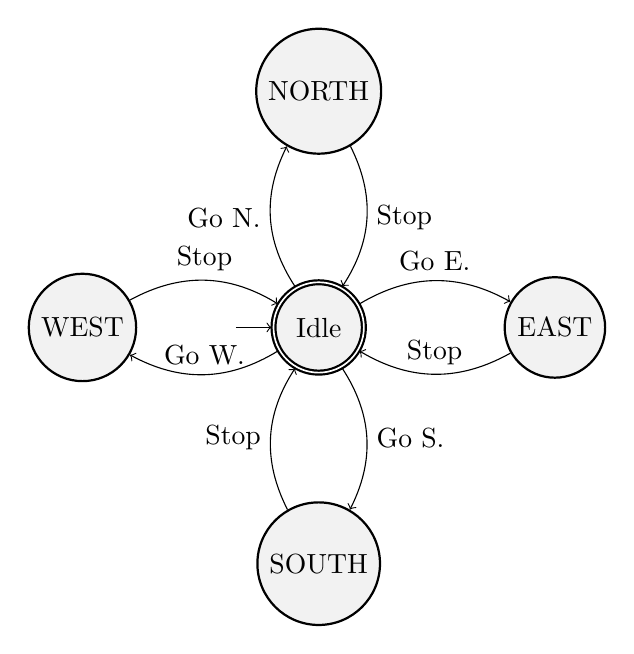
\begin{tikzpicture}
\node[state, initial, accepting] (idle) {$ $ Idle $ $};
\node[state, right of=idle] (east) {EAST};
\node[state, left of=idle] (west) {WEST};
\node[state, above of=idle] (north) {NORTH};
\node[state, below of=idle] (south) {SOUTH};

\draw 	(idle) edge[bend left, above] node{Go W.} (west)
		(west) edge[bend left, above] node{Stop} (idle)
		(idle) edge[bend left, above] node{Go E.} (east)
		(east) edge[bend left, above] node{Stop} (idle);

\draw 	(idle) edge[bend left, left] node{Go N.} (north)
 		(north) edge[bend left, right] node{Stop} (idle)
 		(idle) edge[bend left, right] node{Go S.} (south)
 		(south) edge[bend left, left] node{Stop} (idle);

%\draw (idle) edge[loop above] node{$E_1$} (q1)
%(q1) edge[above] node{$E_2$} (q2)
%(q2) edge[loop above] node{$E_3$} (q2)
%(q2) edge[bend left, above] node{$E_4$} (q3)
%(q3) edge[bend left, below] node{$E_5$} (q2);
\end{tikzpicture}
\end{document}
